\section{ZÁKLADY A TEORIE PŘESNÉHO NÁVRHU S OHLEDEM NA SOUBĚH PARAMETRŮ PRVKŮ INTEGROVANÉHO OBVODU}
Normální rozložení, Gaussova křivka, směrodatná odchylka, metoda Monte Carlo, princip superpozice (příklad součtu výstupních proudů z proudových zrcadel zatížených chybou souběhu)
\subsection{Normální rozložení}
Normální rozdělení neboli Gaussovo rozdělení je jedno z nejdůležitějších rozdělení pravděpodobnosti spojité náhodné veličiny. (Slovo „normální“ zde není použito v nejběžnějším smyslu „obyčejné, běžné“, ale znamená „řídící se zákonem, předpisem nebo modelem“.) Jeho důležitost ukazuje centrální limitní věta (CLV), jež zhruba řečeno tvrdí, že součet či aritmetický průměr velkého počtu libovolných vzájemně nezávislých a nepříliš „divokých“ náhodných veličin se vždy podobá normálně rozdělené náhodné veličině. Normální rozdělení proto za určitých podmínek dobře aproximuje řadu jiných pravděpodobnostních rozdělení (spojitých i diskrétních), i když v praxi málokteré rozdělení je přesně normální.
\begin{figure}[h]
   \begin{center}
     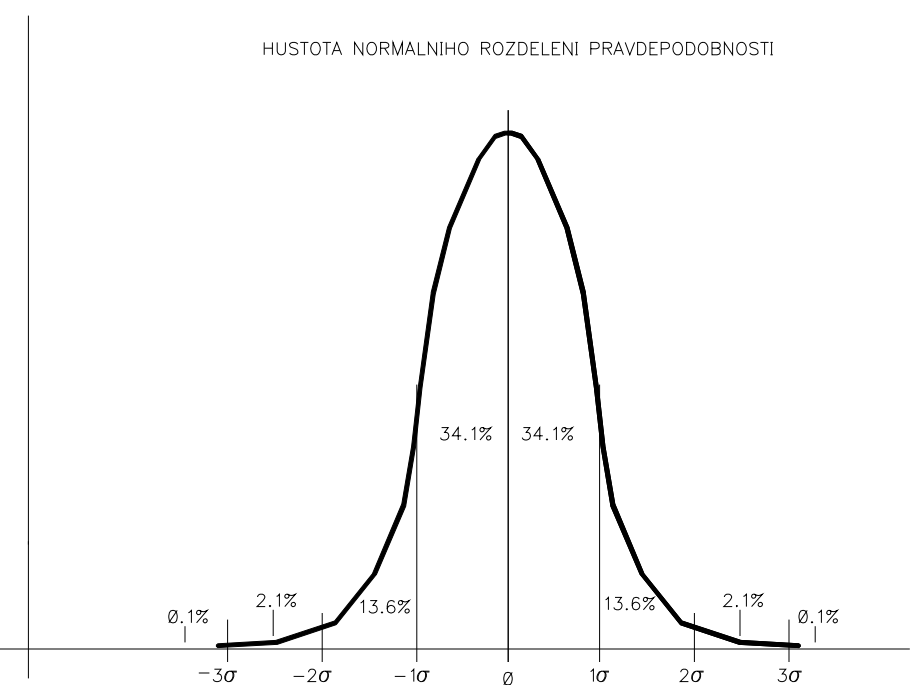
\includegraphics[scale=0.5]{images/normal.png}
   \end{center}
   \caption{Normální rozložení}
\end{figure}

\subsection{Gaussova křivka}
\begin{figure}[h]
   \begin{center}
     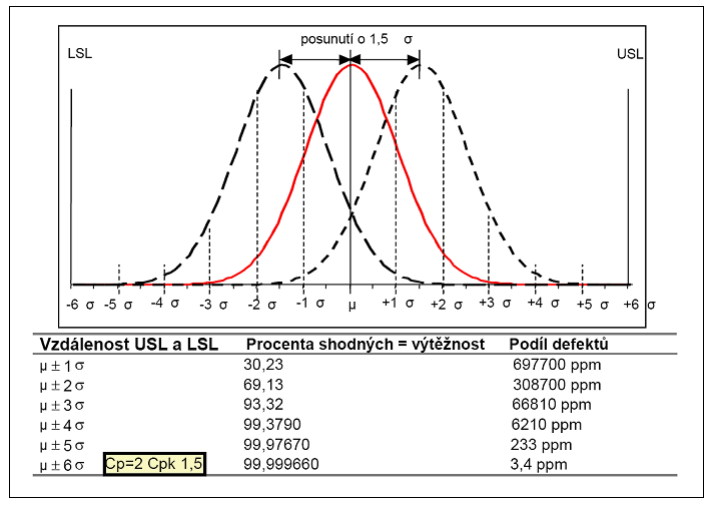
\includegraphics[scale=0.5]{images/Normal1.png}
   \end{center}
   \caption{Znázornění vlivu posunu procesu na ppm}
\end{figure}
\begin{figure}[h]
   \begin{center}
     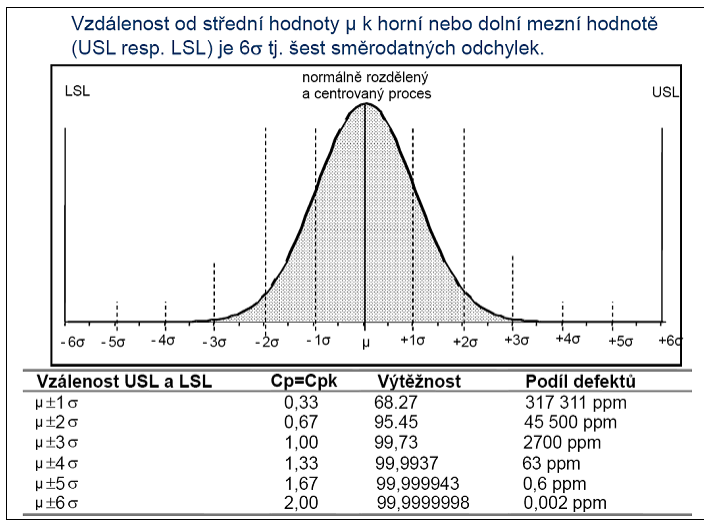
\includegraphics[scale=0.5]{images/Normal2.png}
   \end{center}
   \caption{Vycentrovaný proces a vliv na ppm}
\end{figure}
\subsection{Směrodatná odchylka}
Směrodatná odchylka, podobně jako rozptyl, určuje jako moc jsou hodnoty rozptýleny či odchýleny od průměru hodnot. Směrodatná odchylka je rovna odmocnině z rozptylu.
\begin{equation}
\sigma = \sqrt{var(X)}
\end{equation}
\begin{figure}[h]
   \begin{center}
     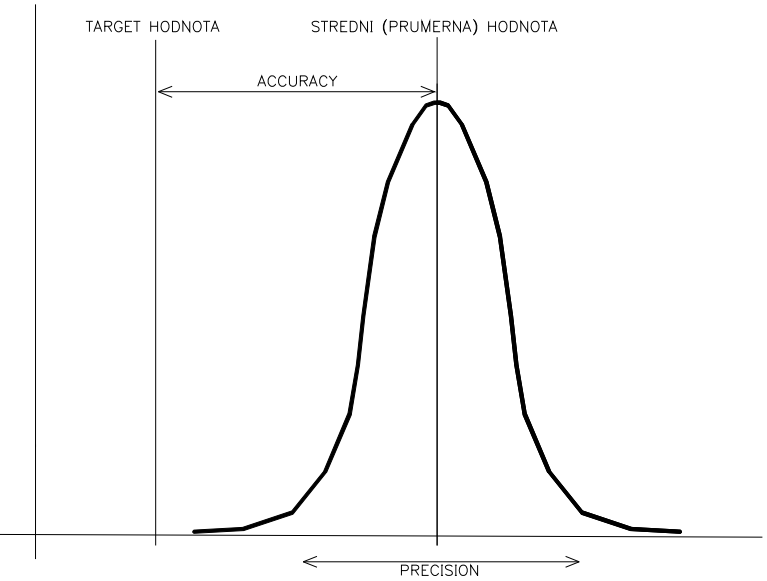
\includegraphics[scale=0.5]{images/Smer.png}
   \end{center}
   \caption{Směrodatná odchylka}
\end{figure}
\subsection{Metoda Monte Carlo}
Metoda je využívána zejména pro výpočet integrálních hustot pravděpodobnosti spojitých náhodných veličin, zejména vícerozměrnýćh, kde běžné metody nejsou efektivní. Tato metoda má široké využití od simulací náhodných experimentů přes numerickou integraci určitých integrálů po numerické řešení diferenciálních rovnic.

Výhodou je jednoduchá implementace, nevýhodou poměrně malá přesnost
\begin{equation}
err = \sqrt{\frac{B}{N}}
\end{equation}
kde N je počet náhodných experimentů a B je konstanta, vyjadřující povahu konkrétního příkladu (pro zvýšení přesnosti výsledku o jeden řád je nutné zvýšit počet simulací alespoň o dva řády).

\subsection{Princip superpozice}
Máme systém, který je charakterizován nějakou veličinou Q (např. offset, výstupní napětí,..). Chyba veličiny Q je dána několika dílčími nekorelovanými chybami uvnitř tohoto systému. Celková chyba veličiny Q se počítá tak, že se postupně vyjádří vliv každé dílčí chyby na veličinu Q, při tom se ostatní dílčí chyby zanedbají - položí rovno 0. NAkonec se vlivy všech dílcích chyb nekorelovaně sečtou a tím se získá celková chyba (rozptyl) veličiny Q.

\subsection{Příklad součtu výstupních proudů z proudových zrcadel}

\begin{figure}[h]
   \begin{center}
     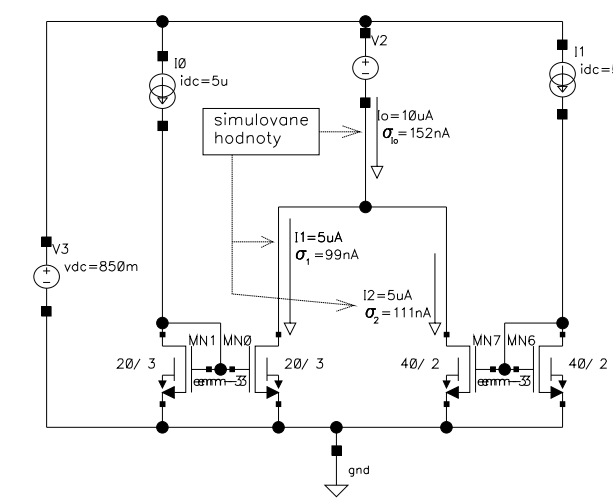
\includegraphics[scale=0.5]{images/Chyba_Souctu.png}
   \end{center}
   \caption{Chyba součtu dvou veličin}
\end{figure}

Mějme dvě veličiny I\textsubscript{1} a I\textsubscript{2}, které jsou vzájemně nekorelované (nijak na sobě nezávisí). Proud I\textsubscript{1} nikterak nezávisí na porudu I\textsubscript{2} a naopak. Velikost těchto proudů je zatížena chybou ($\sigma$\textsubscript{1} a $\sigma$\textsubscript{2}).

Chyba $\sigma$ součtu proudů se potom vypočítá jako:
\begin{equation}
\sigma = \sqrt{\sigma_{1}^{2}+\sigma_{2}^{2}}
\end{equation}

Při sčítání nekorelovaných veličin je jedna důležitá vlastnost. Pokud je jedna veličina menší než 1/2 největší veličiny, ve výsledku se téměř neprojeví (dá se zanedbat), protože zvýší výslednou hodnotu jen asi o desetinu.

Mějme: x\textsubscript{1}=1 a x\textsubscript{2} = 0,5. Potom:
\begin{equation}
\sigma = \sqrt{\sigma_{1}^{2}+\sigma_{2}^{2}}=\sqrt{1^{2}+0,5^{2}}=1,12\doteq 1
\end{equation}
